\documentclass[12pt,a4paper,onecolumn,oneside,final]{report}

\usepackage[dthesis]{thesis-ict-en}
\affiliation{}{Department of Information and Communications Engineering\\School of Engineering}
\usepackage[bottom=1.5in]{geometry}

% ----------------------------------------------------------------------
% packages
% ----------------------------------------------------------------------
\usepackage[ipaex]{pxchfon}
\usepackage[utf8]{inputenc}
\usepackage[english]{babel}
\usepackage{setspace}
\usepackage{multirow}
\usepackage{times}
\usepackage{amsmath}
\usepackage{amsfonts}
\usepackage{comment}
\usepackage{enumitem}
\usepackage{listings}
\usepackage[table]{xcolor}
\usepackage{booktabs}
\usepackage{cleveref}
\usepackage[dvipdfmx]{graphicx}
\usepackage{import}
\usepackage[labelformat=simple,labelfont=bf]{subcaption}
\usepackage{natbib}
\usepackage{float}
\usepackage{url}
% \usepackage{hyperref}
% \usepackage{cite}

% ----------------------------------------------------------------------
% meta-data
% ----------------------------------------------------------------------
\year{2023}
\date{September 2023}

\advisorA{NANBAA Wan}
\advisorAjobtitle{Professor}
% When there are two supervisors, please use the following:
\advisorB{NANBAA Tsuu}
\advisorBjobtitle{Assoc. Professor}

\title{Title}
\studentid{00D00000}
\author{MABUSHII Sugiru}

% ----------------------------------------------------------------------
% Options
% ----------------------------------------------------------------------
% 参照:https://qiita.com/Hdan/items/8c59a7e0a3215ae32d74
\crefname{chapter}{Chapter}{Chapters}
\creflabelformat{chapter}{#2#1#3}
\crefname{section}{Section}{Sections}
\creflabelformat{section}{#2#1#3}
\crefname{equation}{Equation}{Equations}
\crefname{figure}{Figure}{Figures}
\crefname{table}{Table}{Tables}
\crefname{appendix}{Appendix}{Appendices}
\renewcommand{\figurename}{\textbf{Figure}} 
\renewcommand{\tablename}{\textbf{Table}}
\renewcommand{\thetable}{\arabic{chapter}.\arabic{table}}
\renewcommand{\thefigure}{\arabic{chapter}.\arabic{figure}}
\renewcommand{\thesubfigure}{(\alph{subfigure})} % subcaption でなくここで()をつける
\newcommand{\crefpairconjunction}{ and }
\newcommand{\crefrangeconjunction}{ from }
\newcommand{\crefmiddleconjunction}{, }
\newcommand{\creflastconjunction}{, and }
\captionsetup[figure]{labelsep=colon,labelfont=bf}
\captionsetup[table]{labelsep=colon,labelfont=bf}
\definecolor{gray90}{gray}{0.9} % https://texblog.org/2011/09/02/coloring-every-alternate-table-row/
\lstset{basicstyle=\ttfamily}

% ----------------------------------------------------------------------
% cover and table of contents
% ----------------------------------------------------------------------
\begin{document}

\abstract{こんにちは Hogehoge, こんにちは Hogehoge, こんにちは Hogehoge, こんにちは Hogehoge, こんにちは Hogehoge, こんにちは Hogehoge, こんにちは Hogehoge, こんにちは Hogehoge, こんにちは Hogehoge, こんにちは Hogehoge, こんにちは Hogehoge, こんにちは Hogehoge, こんにちは Hogehoge, こんにちは Hogehoge, こんにちは Hogehoge, こんにちは Hogehoge, こんにちは Hogehoge, こんにちは Hogehoge, こんにちは Hogehoge.}
\maketitle
\setcounter{page}{1}
\renewcommand{\thepage}{\roman{page}}
\setcounter{tocdepth}{1}
\tableofcontents
\listoffigures
\listoftables
\clearpage

% ----------------------------------------------------------------------
% content (内容)
% ----------------------------------------------------------------------
\setcounter{page}{1}
\renewcommand{\thepage}{\arabic{page}}
 
\chapter{Introduction}\label{ch:introduction}
Introduction Figure~\ref{fig:ex-fig}. Hoge \cite{devlin-etal-2019-bert}. Table~\ref{tab:ex-tab}.

\begin{figure}[h]
    \centering
    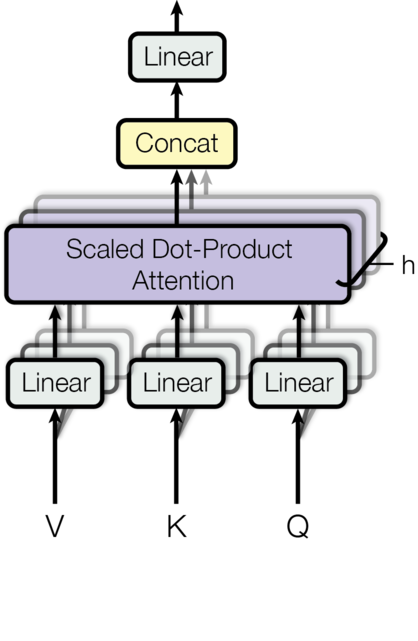
\includegraphics{figures/fig-vkq.png}
    \caption[Example figure]{Example figure.}
    \label{fig:ex-fig}
\end{figure}

\begin{table}[h]
    \centering
    \begin{tabular}{||c c c c||} 
        \hline
        Col1 & Col2 & Col2 & Col3 \\ [0.5ex] 
        \hline\hline
        1 & 6 & 87837 & 787 \\ 
        2 & 7 & 78 & 5415 \\
        3 & 545 & 778 & 7507 \\
        4 & 545 & 18744 & 7560 \\
        5 & 88 & 788 & 6344 \\ [1ex] 
        \hline
    \end{tabular}
    \caption[Example table]{Example table.}
    \label{tab:ex-tab}
\end{table}
\chapter{Related Work}\label{ch:related-work}
\section{hoge}
\subsection{hogehoge}
\section{fuga}
\subsection{fugafuga}
\chapter{Methodology}\label{ch:methodology}
\section{hoge}
    Equation~\ref{eq:ex-eq}.
    \begin{equation}
        \begin{split}
            y &= 2 + 2 \\
            &= 4.
        \end{split}
        \label{eq:ex-eq}
    \end{equation}
\subsection{hogehoge}
\section{fuga}
\subsection{fugafuga}
\chapter{Experiments}\label{ch:experiments}
\section{hoge}
\subsection{hogehoge}
\section{fuga}
\subsection{fugafuga}
\chapter{Results}\label{ch:results}
\section{hoge}
\subsection{hogehoge}
\section{fuga}
\subsection{fugafuga}
\chapter{Conclusion}\label{ch:conclusion}
こんにちは Hogehoge, こんにちは Hogehoge, こんにちは Hogehoge, こんにちは Hogehoge, こんにちは Hogehoge, こんにちは Hogehoge, こんにちは Hogehoge, こんにちは Hogehoge, こんにちは Hogehoge, こんにちは Hogehoge, こんにちは Hogehoge, こんにちは Hogehoge, こんにちは Hogehoge, こんにちは Hogehoge, こんにちは Hogehoge, こんにちは Hogehoge, こんにちは Hogehoge, こんにちは Hogehoge, こんにちは Hogehoge, 
\chapter*{Publication}
\addchapter{Publication}

\begin{itemize}[label={}, leftmargin=*, itemsep=0pt]
    \item \textbf{Journal}
        \begin{itemize}[label=$\bullet$, leftmargin=*, itemsep=0pt]
            \item 
            \item 
        \end{itemize}
    \item \textbf{Conference}
        \begin{itemize}[label=$\bullet$, leftmargin=*, itemsep=0pt]
            \item 
            \item 
        \end{itemize}
\end{itemize}
\chapter*{Acknowledgement}
\addchapter{Acknowledgement}

Thank you. ありがとうございます。



%% original citation style
% \bibliographystyle{junsrt}
%% acl citation style
\bibliographystyle{plainnat}
\bibliography{bib/anthology,bib/main} 

\appendix

\chapter{Implementation}\label{ch:appx:implement}
こんにちは Hogehoge, こんにちは Hogehoge, こんにちは Hogehoge, こんにちは Hogehoge, こんにちは Hogehoge, こんにちは Hogehoge, こんにちは Hogehoge, こんにちは Hogehoge, こんにちは Hogehoge, こんにちは Hogehoge, こんにちは Hogehoge, こんにちは Hogehoge, こんにちは Hogehoge, こんにちは Hogehoge, こんにちは Hogehoge, こんにちは Hogehoge, こんにちは Hogehoge, こんにちは Hogehoge, こんにちは Hogehoge
\begin{figure*}[ht]
    \centering
    
\includegraphics[width=0.5\textwidth]{figures/meme.jpg}
    \caption{ミーム.}
    \label{fig:appx:meme}
\end{figure*}

\chapter{\cref{ch:results} Details}\label{ch:appx:result-detail}
こんにちは Hogehoge, こんにちは Hogehoge, こんにちは Hogehoge, こんにちは Hogehoge, こんにちは Hogehoge, こんにちは Hogehoge, こんにちは Hogehoge, こんにちは Hogehoge, こんにちは Hogehoge, こんにちは Hogehoge, こんにちは Hogehoge, こんにちは Hogehoge, こんにちは Hogehoge, こんにちは Hogehoge, こんにちは Hogehoge, こんにちは Hogehoge, こんにちは Hogehoge, こんにちは Hogehoge, こんにちは Hogehoge
\begin{table}[h]
\centering
\begin{tabular}{|c|c|}\hline
    \textbf{Animal} & \textbf{Sound} \\\hline
    Cow & Moo \\\hline
    Sheep & Baa \\\hline
    Cat & Meow \\\hline
    Dog & Woof \\\hline
    Chicken & Cluck \\\hline
\end{tabular}
\caption{Animal sounds}
\label{tab:appx:animal-sound}
\end{table}
\end{document}